\documentclass{article}
\usepackage[utf8]{inputenc}
\usepackage[english,brazilian]{babel}
\usepackage[editing]{coop-writing}
\usepackage[backend=biber,style=authoryear,
natbib]{biblatex}
\usepackage{graphicx} % includegraphics
\usepackage{csquotes} %enquote, textquote...
\usepackage{enumitem} % noitemsep, nolistsep
\setlist[itemize]{noitemsep}
\setlist[itemize]{nolistsep}
\setlist[enumerate]{noitemsep}
\setlist[enumerate]{nolistsep}
\renewcommand*{\mkcitation}[1]{ #1}
\usepackage{outlines}
\addbibresource{ec.bib}
\cwnamedef{xexeo}{red}{Xexéo}
\setlength{\parskip}{0.5em}
\title{Dicas de Escrita de Artigos Científicos}
\author{Geraldo Xexéo}
\date{Junho de 2021}

\begin{document}

\maketitle

\tableofcontents

\section{Introdução}
\cwmain{Este texto apresenta dicas de escrita de artigos científicos, em especial para Computação, com foco em brasileiros que tem que escrever em inglês.} Essas dicas foram coletadas a partir da leitura de vários livros, artigos e sites que serão indicados ao longo do texto.

O fato de eu escrever este documento não significa que eu escreva bem, mas que eu me esforço para isso e que, com o tempo, adquiri um conhecimento que me permite, principalmente, criticar o meu próprio trabalho e o dos outros como revisor.

As dicas aqui colocadas tem esse objetivo específico e, em geral, não são perfeitamente adequadas para outras formas de escrita.

\cwmain{Este texto está sendo distribuído com o pacote \texttt{coop-writing}, onde coloquei marquei com o comando \texttt{cwmain} os inícios de parágrafos para demonstrara técnica de construí-los a partir de uma ideia única que os inicia.} Algumas vezes, não consegui achar a melhor forma de fazer isso, outras vezes, como nas regras e dicas mais diretas, isso não é possível.

\section{Não é fácil escrever}

\cwmain{Escrever não é fácil.} Um iniciante pode acreditar que textos são escritos uma vez e estão prontos. Não é verdade. Textos de qualidade foram escritos e reescritos, revisados e editados.

\cwmain{É necessário reescrever e revisar muitas vezes um texto para que fique bom}, e nem cito a palavra ótimo\footnote{Como diz o ditado popular ``O ótimo é inimigo do bom''. A interpretação correta desse ditado é que se tentamos ser ótimos podemos não conseguir ser bons.}, para ser aceito por uma revista ou congresso científico. Reescrevemos o texto para ele ficar mais claro e  compreensível. Revisamos o texto para ele ficar correto ortográfica, gramática e estilisticamente.

\cwmain{Escrever em uma segunda língua, como é para nós o inglês, é ainda mais difícil.} Principalmente para quem não viveu por um tempo razoável falando em inglês diariamente. Temos dificuldade com as palavras mais adequadas, com as estruturas e com a forma de expressar nosso pensamento que vão muito além daquelas que enfrentamos em inglês.

\cwmain{Para diminuir a dificuldade de escrever em inglês é \textbf{importante ler em inglês}.} Isso trará justamente o conhecimento da ortografia, da gramática e do estilo adequado. Se o escritor não lê na língua que escreve, não tem uma base de exemplos suficiente para poder criar o seu texto.


\section{O que é estilo de escrita?}

\cwmain{Um estilo de escrita é uma forma de expressar as ideias através de texto.} Um texto é composto de palavras ordenadas em uma sequência específica, e possui um significado. Se você se lembra do seu curso fundamental e médio sabe que existe a ortografia e a gramática, que falam das palavras e da estrutura do texto. Além disso, temos o significado, ou semântica. Também temos a pragmática, que analisa o texto dentro de um contexto. Mais além, temos um efeito da forma como as ideias são apresentadas, talvez fortemente estético, que agrada mais, ou menos, seus leitores, ou torna mais fácil, ou mais difícil, a leitura.

\cwmain{O estilo de escrita pode ser analisado de várias formas}, como em relação a um escritor, como o estilo de escrita de José Saramago, como em função de uma nacionalidade ou época, o estilo da poesia barroca, etc. Uma das formas é em função do objetivo geral do texto, como informar, descrever, etc., caracterizando um tipo de estilo. Na escrita científica, revistas e congressos também tem estilos próprios.

\cwmain{Alguns tipos de estilo reconhecidos são o expositivo, o descritivo, o persuasivo e o narrativo}\citep{jeffrey:2016}.
Como podem ver um mesmo texto pode possuir vários tipos de estilos.

\cwmain{Para escolher um estilo de escrita é necessário conhecer o seu objetivo e quem são os seus leitores.} A audiência tem expectativas que devem ser atendidas, e, quando quebradas, podem deixar o leitor desconcertado e evitar que eles leiam seu artigo.

\cwmain{Existem regras, ou pelo menos padrões, tradicionais de estilo em escrita científica de artigos em inglês.} Por exemplo, devemos evitar  a voz passiva.

\cwmain{Só podemos quebrar essas regras se sabemos muito bem o que estamos fazendo.}
Bons autores tem estilo próprio que quebram algumas regras, ou mesmo todas, porém devemos considerar duas coisas: primeiro, não estamos fazendo literatura, segundo, se você está lendo esse texto, provavelmente ainda não chegou no nível de experimentar com os estilos.

\cwmain{Alguns autores procuram formas excessivamente complicadas de se expressar em artigos científicos}. As sentenças na lista a seguir usam estilos diferentes para passar a mesma ideia geral. Eu exagerei ao criar esses exemplos, mas é a sensação que tenho ao ler alguns artigos.
\begin{itemize}
    \item Foi necessário, por mim, convocar o competente discente João para auxiliar a remover mais rapidamente os entraves que obstaculavam a sua inscrição nesse instituto educacional.
    \item João, um valoroso aulista, foi convocado por mim para deslindar alguns empecilhos para sua matrícula.
    \item Chamei João, que é um bom aluno, para resolver problemas com sua matrícula.
\end{itemize}



\cwmain{Devemos procurar um estilo que facilite a leitura.} Para mim isso significa, por exemplo:
\begin{itemize}
    \item usar inglês simples, com palavras que não precisam ser buscadas em um dicionário;
    \item construções diretas das sentenças, que não devem ser longas ou cheias de vírgulas, e
    \item evitar jargões, principalmente de outras áreas que não a tratada no artigo.
\end{itemize}

 \cwmain{Eu gosto da ideia de usar listas explícitas.}
 É um estilo pessoal, e não é um inglês muito rico, porém elas facilitam a visualização de ideias e exemplos, sendo muito melhores para isso do que colocar dois pontos e seguir com uma lista de itens separados por vírgulas.

 \cwmain{Essas listas podem ser transformadas facilmente em parágrafos ou incluídas dentro de um texto, seguindo o dois pontos.} Por exemplo, se cada item da lista precisar de uma explicação, é possível transformá-los em parágrafos distinto, com palavras de ligação entre os parágrafos como ``First'', e ``Second''. O segundo caso pode ser necessário se falta espaço no artigo.

\subsection{A distância entre o que escrevemos e o que é compreendido}

\cwmain{Existe uma distância muito grande entre o que pensamos e o que vai entender o leitor de nosso texto.} Essa distância pode levar a compreensão errada de nossas ideias.

\cwmain{Como podemos ver pelos exemplos anteriores, a mesma ideia pode ser passada, corretamente, por vários textos.} Do mesmo modo, o mesmo texto pode gerar várias ideias.

\cwmain{A frase ``Vi um homem de binóculo'' mostra como um texto pode ser lido de várias formas.}
Ela permite duas interpretações: eu estava usando um binóculo, ou o homem portava um binóculo. Ela pode ser reescrita de outras formas para evitar essa ambiguidade, por exemplo: \enquote{De binóculo, vi um homem}, \enquote{Eu usava um binóculo quando vi um homem a distância}. Todas essas frases estão corretas, mas a original é totalmente ambígua\footnote{A amiguidade, nesse caso, é gramatical, já que duas estruturas gramaticais podem ser construídas}, não nos permite afirmar, com certeza, se quem estava de binóculo era eu, ou o homem. A segunda, dependendo de onde é usada, poderia ainda dizer que quem estava usando o binóculo era o homem, por exemplo se respondendo a questão ``Você viu alguém com binóculo ou chapéu?''.
Na terceira tudo está mais claro e é difícil escolher um contexto onde não represente exatamente o fato de que eu estava de binóculo e não o homem.

\cwmain{A Figura \protect\ref{fig:tr1} mostra a distância entre o que pensamos e o que o leitor vai interpretar}.

\begin{figure}
    \centering
    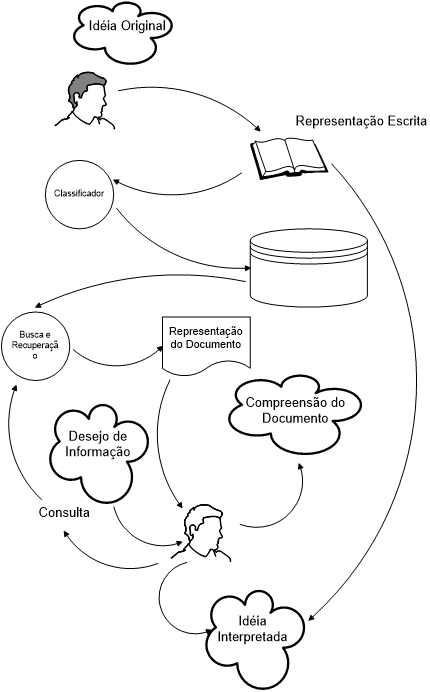
\includegraphics[height=12cm]{imagens/textretrieval.png}
    \caption{Da ideia do autor a ideia do leitor, muito pode acontecer. (desenho do autor)}
    \label{fig:tr1}
\end{figure}

\section{O Problema de Múltiplos Autores}

\cwmain{Em um artigo de vários autores, eles devem se organizar em torno de um estilo único.} Uma das dificuldades de escrever artigos em co-autoria é normalmente a mistura de estilos. Escolhendo, ou mesmo se submetendo a um estilo único, os autores evitam que o leitor tenha a sensação de estar lendo uma colagem ou colcha de retalhos.

\section{O Objetivo do Texto Científico}

\cwmain{O objetivo do texto científico é passar uma ideia complexa de forma compreensível para uma audiência internacional, onde a maioria sabe o inglês como segunda língua}. Essa ideia deve adicionar algo ao corpo de conhecimento de uma área de pesquisa.

\cwmain{A norma, então, deveria ser escrever textos simples.} Entretanto, cada revista ou congresso costuma adotar um estilo diferente, muitas vezes  rebuscado ou que exige forte conhecimento de notações e jargões pré-estabelecidos.

Minha hierarquia de objetivos é a seguinte:
\begin{enumerate}
    \item Divulgar minha pesquisa ou proposta;
    \item Permitir que sejam facilmente compreendidas;
    \item Facilitar ao leitor a leitura completa do artigo, e
    \item Convencer o leitor que minhas propostas e opiniões estão corretas.
    \item Atender as regras do meio de publicação.
\end{enumerate}

Para isso precisamos atingir algumas qualidades:
\begin{itemize}
    \item A \textbf{necessidade}, não colocando no texto material desnecessário. Tudo que está no texto deve ter uma finalidade.
    \item A \textbf{concisão}, usando o menor texto possível que seja adequado ao contexto.
    \item A \textbf{clareza}, não criando construções convolutas.
    \item A completude ou fechamento do texto, permitindo que o leitor, com o \textit{background} adequado, compreenda o texto.
\end{itemize}

\cwmain{ A audiência de um artigo possui um conhecimento específico que não devemos replicar no artigo.} Esse \textit{background}, permite tratar de assuntos sem que tenhamos de reconstruir a história da área, o que é desnecessário e torna o artigo aborrecido.


\section{Seja Forte no Início}

\cwmain{Devido a uma ideia errônea que a introdução deve partir de algo muito geral, muitos autores começam seu artigo com um texto que não traz nenhuma informação nova}, logo não atiça a curiosidade do leitor, nem o prepara para o que está por vir.

\citeauthor{Knuth:1997} dizem:

\textquote[{\citep{Knuth:1997}}]{The opening paragraph should be your best paragraph, and its first sentence should
be your best sentence. If a paper starts badly, the reader will wince and be resigned to
a difficult job of fighting with your prose. Conversely, if the beginning flows smoothly,
the reader will be hooked and won’t notice occasional lapses in the later parts.}

\cwmain{Apoiado neste texto de \protect\citet{Knuth:1997}, eu acredito que o melhor primeiro parágrafo diz o que o texto apresenta.} Por exemplo, este é um primeiro parágrafo de um artigo que estou escrevendo:

\textquote{This article defends that heroic journeys are an effective way to help female students to overcome barriers in STEM education.
It also shows how to build courses based on heroic journeys, taking into account motivational theories, self-regulation of learning, and project based learning. Finally, it describes the Heroine's Learning  Journey and a framework that  supports its use in the development of online courses.}\xexeo{defends ainda é meio fraco, mas por enquanto é a versão mais forte que conseguimos.}

Porém, algumas vezes, o estilo é ditado fortemente pela revista ou pela área de atuação, por exemplo, esse texto segue uma abordagem totalmente diferente.

\textquote{Let $G = (V,E)$ be a simple undirected graph, with a set of vertices $V$ and a set of edges $E$. Denote by $E(C) \subset E$, $C \subset V$, the edges of $G$ with both endpoints in $C$ and by $G(C) = (C,E(C))$ the subgraph in $G$ induced by $C$. If $G(C)$ is complete, $C$ is called a clique. An \textit{Edge Clique Cover} (ECC) of $G$, in turn, is defined as a set of cliques ${C_1,...,C_k}$, $k \geq 1$, for which $E = \bigcup_{i=1,..,k}E(C_i)$ applies, i.e., a set of cliques for which their induced edges \textit{cover} (contain) all edges in $E$. The smallest cardinality possible for such a set, $\kappa$, is called the ECC number of $G$ and the ECCP is to find an ECC with cardinality exactly $\kappa$.}\footnote{Texto gentilmente cedido pelo Douglas}

E, como um exemplo que considero um contra-exemplo do que um bom primeiro parágrafo, um artigo que apresentei com outros autores apresenta o seguinte texto como primeiro parágrafo:

\textquote{Game design and development turned out to be a legitimate profession and industry. There are undergraduate and graduate courses in Game Design, Art, Programming and all others aspects related to this endeavor. Some schools even adopted the term Game Engineering, recognizing that games are engineering artifacts}

Qual a diferença entre os 3 parágrafos em função de atrair o leitor?

O primeiro deixa claro o que é o artigo, de forma explícita, fazendo com que o leitor decida imediatamente se está interessado ou não. O segundo deixa claro quase de forma implícita que vai tratar do problema do ECCP, porém segue uma prática dos artigos da área. Já o terceiro deixa o leitor ainda sem saber o que é o artigo, se perdendo em generalidades.

A menos de questões da revista em que vai ser publicado, eu começaria o segundo parágrafo com algo como \enquote{This article introduces a new and faster algorithm to solve Edge Clique Cover Problem (ECCP)}.

Como esse é um texto pessoal, eu aceito que alguns autores, ou mesmo a maioria deles use uma abordagem \textit{top-down} em sua introdução para abordar o seu problema, porém eu prefiro dizer, e saber quando estou lendo, para que veio o artigo. Sinceramente, eu normalmente pulo os textos introdutórios que seguem o padrão do terceiro parágrafo mostrado.

\subsection{Primeiro Parágrafo da Seção}

Essa ideia também se aplica ao primeiro parágrafo de uma seção. A seguir mostro um parágrafo que inicia uma seção no mesmo artigo:

\textquote{In this section we show that there is a low participation of female students in STEM courses, due to the multiple challenges they must face to participate in them. Furthermore, we show that this is considered a worldwide problem, and that there are many initiatives trying to solve it.}

Lendo esse parágrafo o leitor não precisa mais ler o resto da seção, a não ser que queira detalhes. Tudo que a seção diz, em três subseções e cinco páginas está resumido aí.

\subsection{A Técnica da Primeira Frase}

\cwmain{A primeira frase do parágrafo deve apresentar a ideia que justifica sua existência.} Em geral, cada parágrafo de um artigo deve apresentar uma ideia, e uma ideia apenas . Para construir parágrafos fortes, essa ideia deve estar resumida na primeira frase. O resto do parágrafo deve explicá-la ou justificá-la.

\cwmain{Dessa forma, o leitor que dá uma ``leitura diagonal'' pode ler apenas as primeiras frases e ter uma ideia bem clara do artigo.} Isso é uma enorme vantagem, pois muitos leitores fazem isso, logo aumenta o seu público.

\section{Último Parágrafo da Seção}

\cwmain{No último parágrafo da seção eu defendo um resumo da mesma, mesmo que pareça em conteúdo com o primeiro parágrafo.}  De certa forma, devemos garantir que o leitor não se perdeu ao longo da leitura e vai passar para a próxima parte do artigo com a ideia que queríamos consolidada.

\cwmain{É importante dizer a mesma coisa de outra forma, não repetindo o texto}, mas tentando mostrar como, a partir da seção, podemos chegar as conclusões desejadas. \citet{Knuth:1997} dizem:

\textquote[\citep{Knuth:1997}]{Try to stat things twice, in complementary ways, especially when giving a definition. This reinforces the reader's understanding.}

Existem, porém, exceções, por exemplo, se a seção é pequena, então pode não ser necessário. Mas se ela é pequena, por que existe?


\section{O uso do tempo verbal}

\cwmain{Os textos devem ser escritos no presente}, a menos de eventos que ocorreram no passado, ou que ocorrerão no futuro.

\cwmain{É possível também escolhar um modelo passado/presente/futuro.} Nesse caso, o trabalho anterior ao seu é descrito no passado, o seu no presente e os trabalhos propostos no futuro.

\cwmain{É importante escolher um mesmo tempo verbal para todas as citações}. Se ``João (1995) propôs'', o que eu acho mais adequado, então ``Maria (2020) defendeu''. Porém é razoável pensar que as citações que fazemos são a artigos existentes hoje, então ``João (1995) propõe'' e ``Maria (2020) defende'' é razoável.

\cwmain{O uso do passado nas citações facilita construir uma linha de tempo das publicações}, e parece mais adequado. Por exemplo: ``Mary (1995) had initially proposed cheese and bread sandwiches, but later, in 2000, she introduced ham in them (Mary de Kooc, 2000)''. Esse texto, com tudo no presente, não ficaria muito bom.



\cwmain{Todo o trabalho de sua autoria apresentado deve estar no presente}, a não ser que parte do texto seja uma narrativa, o que é raro na Computação. Estudos de caso, porém, podem cair nessa situação e ser descritos no passado.

\section{Regras Simples}

\subsection{Práticas Obrigatórias}

Essas regras são, na verdade, gramaticais. Se você erra nesse nível, vai ter problemas sérios para ter o texto aceito para publicação.

Esses erros são fáceis de encontrar em uma revisão. Na verdade, todos cometemos esses erros, principalmente quando interrompidos no meio do processo de escrever uma frase. ou quando não somos fluentes na linguagem. Porém, é importante estar atento e trabalhar frase por frase para detectá-los.

Se estivermos em dúvida sobre algumas dessas, como se não sabemos qual o tempo certo, podemos reescrever a frase, buscar explicações de gramática na Web, ou usar sofwares específicos, tratados na seção \ref{sec:software}.

\begin{outline}
    \1 Não separe o sujeito do verbo por vírgulas.
    \2 \sout{My professor John, wrote me a recommendation letter}.
    \1 O verbo e o sujeito \textbf{devem concordar} em gênero, número e pessoa.
    \2 \sout{John and Julia is my favorite students}.
        \3 Ask: Who is? John and Julia. They are 2, so the verb must be in the plural (Who are?).
    \2 John and Julia are my favorite students.
    \2 Em inglês, verbos não variam com o gênero.
\end{outline}

\subsection{Práticas a evitar}
\begin{outline}
\1 \textbf{Evite a voz passiva.}
\2 Em inglês a voz passiva é considerada uma forma fraca de passar ideias. Podemos perceber, lendo uma sentença na voz passiva, que ela também exige um racionío mais longo, logo complica o entendimento do texto. Em português costumamos usar muita voz passiva.
\1 Evite adjetivos.
\1 Evite o uso de parênteses.
\1 Evite o excesso de vírgulas, e as mudanças da ordem natural da sentença.
\1 Evite sentenças muito longas.
\1 Evite deixar o sujeito muito longe do verbo.
\2 Além de dificultar a compreensão, leva a errar a concordância verbal.
\end{outline}

\subsection{Opções}

\begin{outline}
\1 \textit{which} vs \textit{that}
\2 Se vem depois da vírgula é \textit{which}, se vem sem vírgula é \textit{that}.
\end{outline}

\subsection{Expressões em Inglês}

\cwmain{Algumas expressões comuns em português podem ter traduções bem diferentes em inglês.} A pequena lista a seguir foi retirada de um site da web\footnote{\url{https://www.sk.com.br/sk-conn-words-of-connection-conectivos-do-ingles.html}}.

\begin{outline}
    \1 Por outro lado $\rightarrow$ \textit{on the other hand}.
    \1 Em primeiro lugar $\rightarrow$ \textit{To begin with}
    \1 Na verdade    $\rightarrow$ \textit{Actually}
    \1 Atualmente    $\rightarrow$ \textit{Nowadays} ou \textit{Currently}
    \1 Com objetivo de $\rightarrow$ \textit{In order to/that}
    \1 Sempre que $\rightarrow$ \textit{Whenever}
    \1 Em detrimento/prejuízo de $\rightarrow$ \textit{at the expense of}
\end{outline}


\section{Diferenças Básicas no Inglês}

\begin{outline}
    \1 Começam com em letra minúscula no português mas em letra maíscula no inglês\xexeo{Alguma coisa importante está faltando?}:
    \2 dias da semana, como \textit{Tuesday};
    \2 nomes de mês, como \textit{June};
    \2 nomes de linguagens, como \textit{Esperanto}, e
    \2 nomes ou adjetivos regionais, como \textit{Brazilian} ou \textit{British}.
\end{outline}

\subsection{Falso Cognatos}

\cwmain{Falsos cognatos são palavras semelhantes em duas línguas que não significam a mesma coisa}, como ``library'', que não significa ``livraria'', mas biblioteca.

\cwmain{Devemos estar atentos para a tendência de buscar a palavra mais parecida a uma que desejaríamos usar em português e cair na armadilha de usar um falso cognato.}

\cwmain{Atenção para a a seguir de lista de palavras em inglês que não tem o significado da palavra mais semelhante em português}. Não são as únicas, mas são palavras frequentemente usadas de forma errada.
\begin{itemize}
    \item \textit{Actual} $\rightarrow$ real, e não atual.
    \item \textit{Agenda} $\rightarrow$ pauta do dia. Uma agenda é um \textit{diary}.
    \item \textit{Application} $\rightarrow$ inscrição.
    \item \textit{Attend} $\rightarrow$ participar.
    \item \textit{College} $\rightarrow$ faculdade, mas quando é parte de um nome às vezes a tradução é colégio mesmo.
    \item \textit{Costume} $\rightarrow$ fantasia.
    \item \textit{Data} $\rightarrow$ dados, uma data é \textit{date}.
    \item \textit{Eventually} $\rightarrow$ finalmente, e que sempre acontece. Eventualmente é \textit{occasionally}.
    \item \textit{Fabric} $\rightarrow$ tecido.
    \item \textit{Genial} $\rightarrow$ agradável, amável.
    \item \textit{Intend} $\rightarrow$ pretender, de ter a intenção e não. entender
    \item \textit{Journal} $\rightarrow$ periódico ou revista especializada, jornal é \textit{newspaper}, revista comum é \textit{magazine}.
    \item \textit{Library} $\rightarrow$ biblioteca.
    \item \textit{Notice} $\rightarrow$ notar, perceber. Notícia é \textit{news}.
    \item \textit{Novel} $\rightarrow$ um romance, no caso de livros, ou algo novo e não usual, interessante. Novela é \textit{soap-opera}.
    \item \textit{Patron} $\rightarrow$ bem-feitor, não é patrão.
    \item \textit{Pretend} $\rightarrow$ fingir.
    \item \textit{Prejudice} $\rightarrow$ preconceito.
    \item \textit{Realize} $\rightarrow$ perceber.
    \item \textit{Reclaim} $\rightarrow$ recuperar. Reclamar é \textit{to complain about}.
    \item \textit{Sensible} $\rightarrow$ sensato.
    \item \textit{Ultimately} $\rightarrow$ em última análise. Ultimamente é \textit{lately} ou \textit{recently}.
    \end{itemize}


\section{Comentários sobre métodos de escrita}

\subsection{O Método da Pirâmide de Barbara Minto}

\citet{minto2009pyramid} propõe um método baseado na ideia de uma pirâmide.

\todo{fazer um resumo do método Minto}

\section{Técnicas de Revisão}

\cwmain{A revisão do texto busca corrigi-lo ortográfica, gramática e estilisticamente}, de forma a estar correto conforme os padrões determinados pela revista ou congresso onde será publicado.

\cwmain{A revisão pode ser feita pela simples leitura do texto em busca de erros}, e isso é razoavelmente possível se você possui um grande da língua ou da técnica de uso da língua. Um professor de português, por exemplo, pode fazer uma correção em uma redação e achar grande parte dos erros que estão lá, mas provavelmente, em uma leitura, não achará todos.

\cwmain{O texto científico é bem mais complicado que uma redação, e provavelmente um revisor precisará de mais de uma leitura.} Ainda mais porque uma correção pode levar a necessidade de outras.

\cwmain{Uma lição da Engenharia de Software sobre revisões de software é uma recomendação que dou: faça uma revisão por tema.} Assim leia primeiro o artigo para buscar erros ortográficos, depois para buscar problemas de concordância verbal, depois tente evitar a voz passiva, e siga sofisticando cada vez mais a revisão de forma a identificar os problemas um a um.

\cwmain{Com o hábito, algumas dessas revisões podem ser unificadas}, e com o tempo você será capaz de fazer quase todas em uma vez só.

\cwmain{Lembre-se, porém, que escrever não é fácil, e é importante reescrever e revisar para tornar sua mensagem clara.}

\cwmain{Não tenha medo de reescrever.} Muitos autores acham que o texto, ou parte do texto, ``já está pronto'' e não deve ser mexido. Na verdade, enquanto escrevemos entendemos melhor o que já escrevemos e podemos ter ideias de como melhorar o texto que não devemos deixar passar.

\section{Software}
\label{sec:software}
Grammarly e LanguageTool.

\section{Guia de Leitura}

\printbibliography

\newpage

\listofsubjects

\end{document}
